\documentclass[runningheads]{llncs}
%
\usepackage{xurl}
\usepackage{graphicx}
\usepackage[portuguese]{babel}
\usepackage[utf8]{inputenc}
\usepackage{amsmath}
\usepackage{amssymb}
\usepackage{amsfonts}

\begin{document}
%
\title{Investigação Operacional - Trabalho Prático 1}
\author{Carlos Machado a97114, Gustavo Pereira a96867,
Vasco Oliveira a96361, Cláudio Bessa a97063, Tiago Oliveira a97254}

\institute{Universidade do Minho}

\authorrunning{Carlos \and Gustavo  \and Vasco \and Cláudio \and Tiago}



\maketitle      
\newpage
\section{Formulação do Problema}


O problema em causa surge quando um drone precisa de inspecionar linhas de transporte de energia eléctrica em alta tensão para verificar se há vegetação a interferir com as linhas. Este pode percorrer as arestas (linhas de alta tensão) em qualquer sentido, tendo também possibilidade de viajar pelo ar,\textit{i.e}, sem seguir as linhas de alta tensão.

O objetivo principal deste desafio é fazer com que o drone percorra a menor distância possível, partindo do vértice I e acabando no vértice F, sendo obrigatório percorrer todas as linhas pelo menos uma vez, quer as que estão representadas originalmente no mapa, quer as linhas adicionaremos de modo a formar um caminho euleriano.

O maior número de estudante do grupo é 97254, o que significa que teremos de retirar as arestas C e E do mapa inicial, resultando no mapa que se observa na Figura 1.

\begin{figure}[h]
\centering
\includegraphics[scale=0.45]{drone.png}
\caption{Mapa de linhas de alta tensão, após remoção das arestas C e E.} 
\label{fig:data1}
\end{figure}

\newpage 

\section{Modelo}
Uma vez que pretendemos percorrer todas as arestas do percurso de forma eficiente, podemos observar este problema como um caminho euleriano, onde pretendemos encontrar um percurso para um caminho de forma a passar em todas as arestas uma só vez. Este caminho apenas existe quando os vértices interiores ao mapa têm grau de entrada/saída par, e os vértices que representam o início (I) e o fim (F) do percurso grau ímpar.

Na Figura 2, encontram-se assinalados os vértices onde é necessário aumentar o grau, \textit{i.e}, criar ou duplicar novas adjacências, para tornar o percurso um caminho euleriano. Desta forma, obtemos um problema de programação linear onde procuramos adicionar arestas tentando otimizar o itinerário de modo a minimizar a distância percorrida pelo drone.

\begin{figure}[h]
\centering
\includegraphics[scale=0.25]{arestasgrau.jpg}
\caption{Vértices com grau insuficiente.} 
\label{fig:data2}
\end{figure}

\subsection{Variáveis de decisão}

$xij$: existe ou não uma aresta a unir os vértices $i,j \in \{I,1,2,3,4,6,7,9,10,11,12,F\}$, onde $xij \in \{0,1\}$.

\begin{figure}[h]
\centering
\includegraphics[scale=0.8]{vars.png}
\caption{Variáveis de decisão} 
\label{fig:data3}
\end{figure}

\newpage

\subsection{Parâmetros}

$dij$ : comprimento da aresta que une os vértices i e j.
Os comprimentos de todas as arestas podem ser calculados a partir da seguinte tabela:

\begin{figure}[h]
\centering
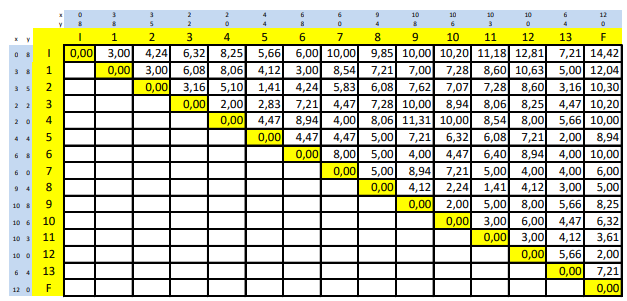
\includegraphics[scale=0.75]{distancias euclidianas.PNG}
\caption{Distancias Euclidianas fornecidas} 
\label{fig:data4}
\end{figure}

\subsection{Função objetivo}
Minimização da distância percorrida pelo \textit{drone}.
\newline \textit{min} : $\sum_{i,j}^{} \in V,  dij  \times    xij,  i < j$

\begin{figure}[h]
\centering
\includegraphics[scale=0.4]{obj_func.png}
\caption{Função objetivo} 
\label{fig:data5}
\end{figure}

\bigskip
De se lembrar que não são incluídas as arestas 5-13 e 13-8 (presentes na tabela de distâncias) na função objetivo uma vez que estas não são contempladas no nosso mapa.

\newpage
\subsection{Restrições}
Cada vértice apenas deve fazer parte de uma só aresta.
\newline $\forall i \in V \wedge  j \in V,  \sum xij = 1, i < j$

\begin{figure}[h]
\centering
\includegraphics[scale=0.65]{restr.png}
\caption{Restrições} 
\label{fig:data6}
\end{figure}


\newpage

\section{Solução ótima}
Introduzimos os modelo criado no LPSolve e descobrimos as arestas a adicionar no
percurso: $I-1; 2-6; 3-4; 7-11; 9-10; 12-F$. O comprimento total das arestas selecionadas é de 18.24\textit{(u.c)} e o comprimento total é de 9999.99\textit{(u.c)}.

\begin{figure}[ht]
\centering
\includegraphics[scale=0.8]{lpsolve result zoom.png}
\caption{Output retornado pelo LPSolve} 
\label{fig:data7}
\end{figure}

\begin{figure}[ht]
\centering
\includegraphics[scale=0.2]{arestasadicionais.jpg}
\caption{Arestas contempladas como solução ótima} 
\label{fig:data8}
\end{figure}

\newpage


\clearpage

\textbf{Exemplo de percurso}: 
\newline $I \rightarrow 4 \rightarrow 3 \rightarrow 2 \rightarrow 1 \rightarrow I \rightarrow 1 \rightarrow 6 \rightarrow 2 \rightarrow 5 \rightarrow 3 \rightarrow 4 \rightarrow 7 \rightarrow 13 \rightarrow 6 \rightarrow 9 \rightarrow 10 \rightarrow 8 \rightarrow 11 \rightarrow 7 \rightarrow 12 \rightarrow F \rightarrow 12 \rightarrow 11 \rightarrow 10 \rightarrow 9 \rightarrow F$

\begin{figure}[h]
\centering
\includegraphics[scale=0.25]{caminho.jpg}
\caption{Exemplo de um possível percurso.} 
\label{fig:data9}
\end{figure}

\clearpage

\section{Validação do modelo}
Mesmo confiando no método utilizado para obter a solução, é necessária uma validação do modelo utilizado. Para isso, recorremos novamente ao LPSolve.

Vimos como um bom método de validação ir removendo, ao nosso modelo, as arestas pertencentes à solução ótima obtida anteriormente uma a uma, obrigando, desta forma, a gerar um novo percurso. Observando o valor dos outputs destas novas soluções, verifica-se que nenhuma delas apresenta um trajeto com comprimento menor do que o obtido no modelo correspondente à solução ótima.

\bigskip
\textbf{Removendo a aresta \textit{I-1}:}

    Arestas da solução: $I-2; 1-6; 3-4; 7-11; 9-10; 12-F$
    
    Comprimento total das arestas selecionadas: 18.24 \textit{(u.c.)} 

\bigskip
\textbf{Removendo a aresta \textit{2-6}:}

    Arestas da solução: $I-2; 1-6; 3-4; 7-11; 9-10; 12-F$
    
    Comprimento total das arestas selecionadas: 18.24\textit{(u.c.)} 
    
\bigskip
\textbf{Removendo a aresta \textit{3-4}:}

    Arestas da solução: $I-1; 2-3; 4-7; 6-9; 10-11; 12-F$
    
    Comprimento total das arestas selecionadas: 19.16\textit{(u.c.)} 

\bigskip
\textbf{Removendo a aresta \textit{7-11}:}

    Arestas da solução: $I-1; 2-6; 3-4; 9-10; 7-12; 11-F$
    
    Comprimento total das arestas selecionadas: 18.85\textit{(u.c.)} 

\bigskip
\textbf{Removendo a aresta \textit{9-10}:}

    Arestas da solução: $I-1; 2-3; 4-7; 6-9; 10-11; 12-F$
    
    Comprimento total das arestas selecionadas: 19.16\textit{(u.c.)} 

\bigskip
\textbf{Removendo a aresta \textit{12-F}:}

    Arestas da solução: $I-1; 2-6; 3-4; 7-12; 9-10; 11-F$
    
    Comprimento total das arestas selecionadas: 18.85\textit{(u.c.)} 


%\begin{figure}[ht]
%\centering
%\includegraphics[scale=1]{rem_xI1.png}
%\caption{Solução sem a aresta I-1.} 
%\label{fig:data10}
%\end{figure}



\end{document}
